\subsection*{Задание 1.3}

\underline{Условие:} Все потоки случайных событий считать пуассоновскими. Если все операторы заняты, звонок теряется. Рассмотреть систему без ограничений на длину очереди. Построить график математического ожидания длины очереди в зависимости от числа операторов (вплоть до числа каналов, соответствующего 1$\%$  отказов в системе без очереди). Построить график, иллюстрирующий коэффициент загрузки операторов. Построить график математического ожидания времени пребывания клиентов в очереди.\par

\underline{Решение:}\par

Для расчета вероятности, при которой операторы не будут заняты, можно воспользоваться формулой 11:\par


\begin{equation} \label{P0}
    P_{0}=\frac{1}{ \sum _{i=0}^{N}\frac{ \lambda ^{i}}{i! \cdot  \mu ^{i}}+\frac{ \lambda ^{N}}{N! \cdot  \mu ^{N}} \cdot  \sum _{k=1}^{\infty} \left( \frac{ \lambda }{N \cdot  \mu } \right) ^{k}} 
\end{equation} \par

Практический интерес будут представлять такие варианты системы, при которых сумма  \(  \sum _{k=1}^{\infty} \left( \frac{ \lambda }{N \cdot  \mu } \right) ^{k}  \) будет сходящейся. Для того, чтобы данная сумма сходилась необходимо, чтобы член  \( \frac{ \lambda }{N \cdot  \mu }  \) был\ меньше единицы. Исходя из начальных условий практический смысл представляет  рассмотрение систем, где  \( N \geq 9. \)  При таких условиях выражение \ref{P0} можно преобразовать к следующему виду:\par

\begin{equation}
 P_{0}=\frac{1}{ \sum _{i=0}^{N}\frac{ \lambda ^{i}}{i! \cdot  \mu ^{i}}+\frac{ \lambda ^{N}}{N! \cdot  \mu ^{N}} \cdot \frac{ \lambda }{N \cdot  \mu - \lambda }}
\end{equation} \par

Для расчета математического ожидания длины очереди можно воспользeмся формулой:\par

  \begin{equation} \overline{Q}=\frac{ \lambda ^{N}}{N! \cdot  \mu ^{N}} \cdot P_{0} \cdot \frac{a}{ \left( 1-a \right) ^{2}}     \end{equation} \par

где  \( a= \frac{ \lambda }{N \cdot  \mu } \) .\par

Для расчета среднего количества занятых операторов можно воспользоваться\\
формулой:\par

\begin{equation}
 \overline{N}=P_{0} \cdot  \left(  \sum _{i=1}^{N}\frac{ \lambda ^{i}}{ \left( i-1 \right) ! \cdot  \mu ^{i}}+ \frac{ \lambda ^{N}}{ \left( N-1 \right) ! \cdot  \mu ^{N}} \cdot \frac{ \lambda }{N \cdot  \mu - \lambda } \right) 
\end{equation} \par

\begin{figure}[H]
	\begin{center}
        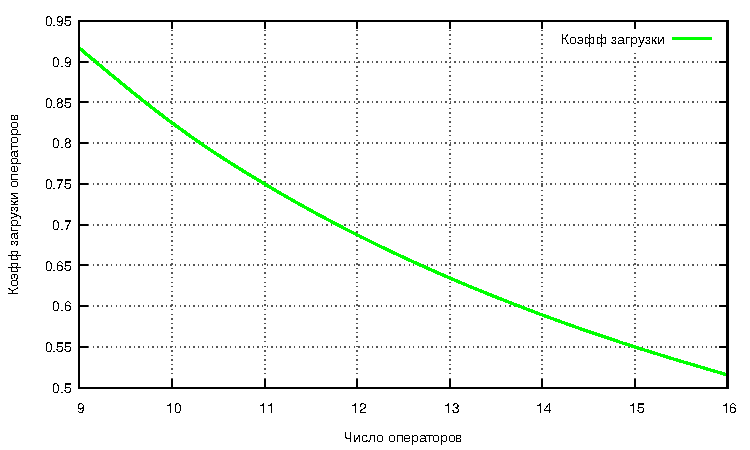
\includegraphics{/z1.3/ninf.pdf}
        \caption{Зависимость коэффициента загрузки операторов от их общего количества}
	\end{center}
\end{figure}


\begin{figure}[H]
	\begin{center}
        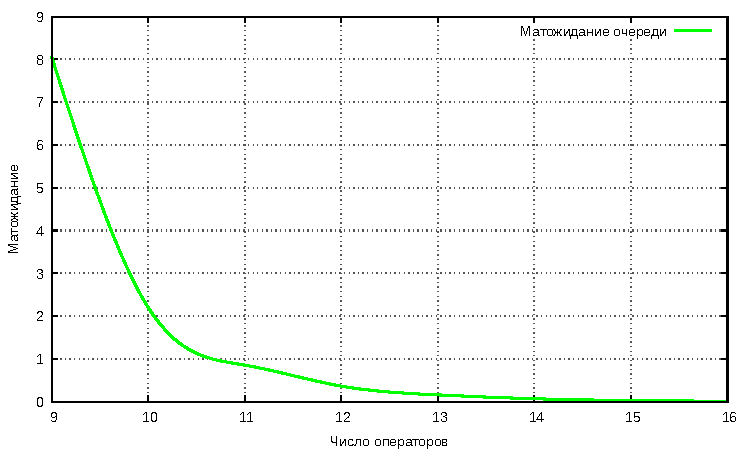
\includegraphics{/z1.3/qinf.pdf}
        \caption{Зависимость математического ожидания длины очереди от количества операторов}
	\end{center}
\end{figure}

\begin{figure}[H]
	\begin{center}
        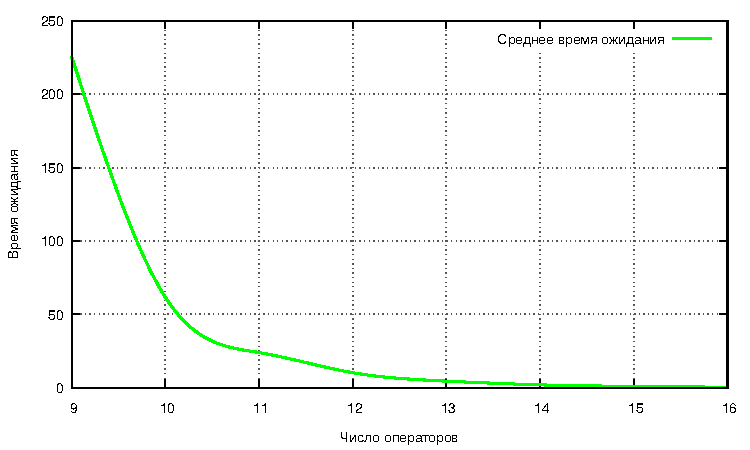
\includegraphics{/z1.3/tinf.pdf}
        \caption{Зависимость математического ожидания времени ожидания в очереди от количества операторов}
	\end{center}
\end{figure}

